%%----------------------------------------------------------------------
\section{お釣りが足りている}
\label{s:お釣り}
%% - - - - - - - - - - - - - - - - - - - - - - - - - - - - - - - - - - -

%%--------------------------------------------------
\subsection{問題}
\label{ssec:お釣り:問題}
%% - - - - - - - - - - - - - - - - - - - - - - - - -

%%--------------------------------------------------
\subsubsection{具体問題}
\label{sssec:お釣り:問題:具体問題}
%% - - - - - - - - - - - - - - - - - - - - - - - - -

ある商人が1個50円のおもちゃを10個売っているとする。
お客は、各々1つずつそのおもちゃを買うとし、
支払いには、100円玉か50円玉でしか支払わないとする。
商人は、最初、お釣り用の50円玉を4枚用意しているとする。
おもちゃ10個が売り切れた時、
商人の手元には50円玉が2枚あった。

この場合、お客が支払った50円玉・100円玉の順序の場合の数は何通りあるか?

%%--------------------------------------------------
\subsubsection{一般化問題}
\label{sssec:お釣り:問題:一般化問題}
%% - - - - - - - - - - - - - - - - - - - - - - - - -

上記の問題で、おもちゃの数を $n$ 個、
最初に用意した50円玉の枚数を $m$ 枚、
最後の残った50円玉の枚数を $l$ 枚とした時、
お客が支払った50円玉・100円玉の順序の場合の数は何通りあるか?


\clearpage
%%--------------------------------------------------
\subsection{解答}
\label{ssec:お釣り:解答}
%% - - - - - - - - - - - - - - - - - - - - - - - - -

%%--------------------------------------------------
\subsubsection{具体問題}
\label{sssec:お釣り:解答:具体問題}
%% - - - - - - - - - - - - - - - - - - - - - - - - -

問題の設定により、
おもちゃが1つ売れる毎に50円玉は1枚増えるか1枚減るかたちで
枚数が変化する。

その様子を表したのが、\figref{fig:S030/Figs/Figure.change.p01}である。
横軸は売れたおもちゃの数、
縦軸が50円玉の数であり、
$(0,4)$ から出発して、$(10,2)$ に至る斜めの碁盤目の経路を辿ることになる。

この内、お釣りの50円玉が足らなくなるのは、図の赤い経路を通る場合である。
つまり、\figref{fig:S030/Figs/Figure.change.p01}で示される碁盤目のうち、
赤い経路を通らない経路の数を数えれば良い。

まず、赤い経路を無視して、全ての碁盤目の経路を数え上げると、
10個の選択肢の中から順不同で4つ選ぶ場合の数であるので、
  %%$$$$$$$$$$$$$$$$$$$$$$$$$$$$$$$$$$$$$$$$$$$$$$$$$$$$$$$$$$$$$$$$$$$$$$
  \begin{eqnarray}
    N_{\text{all}} & = & _{10}C_{4}
  \\
      & = &
        \frac{10!}{4! 6!}
  \\
      & = &
        210
  \end{eqnarray}
  %%$$$$$$$$$$$$$$$$$$$$$$$$$$$$$$$$$$$$$$$$$$$$$$$$$$$$$$$$$$$$$$$$$$$$$$
  
次に、
全て数え上げた中から、お釣りが足らなかった経路を取り上げる。
この時、お釣りが足らなくなった瞬間から、
50円玉の残り数を示す碁盤目を辿る方向を反転させるとする。
すると、
その経路が行き着く先は、
\figref{fig:S030/Figs/Figure.change.p02}のように、
$y=-1$ のところで鏡像にした経路を描く。
よって、その後、$(10,2)$ にたどり着いていた経路は、
この鏡像にした経路の中では、$(10,-4)$ に辿り着く。

そこで、$(0,4)$から$(10,-4)$ に辿る経路を数え上げると、
10個の選択肢の中から1つ順不同で選び出す場合の数であるので、
  %%$$$$$$$$$$$$$$$$$$$$$$$$$$$$$$$$$$$$$$$$$$$$$$$$$$$$$$$$$$$$$$$$$$$$$$
  \begin{eqnarray}
    N_{\text{short}} & = & _{10}C_{1}
  \\
      & = &
        \frac{10!}{1! 9!}
  \\
      & = &
        10
  \end{eqnarray}
  %%$$$$$$$$$$$$$$$$$$$$$$$$$$$$$$$$$$$$$$$$$$$$$$$$$$$$$$$$$$$$$$$$$$$$$$

  %%$$$$$$$$$$$$$$$$$$$$$$$$$$$$$$$$$$$$$$$$$$$$$$$$$$$$$$$$$$$$$$$$$$$$$$
  \begin{eqnarray}
    N_{\text{ans}} & = & N_{\text{all}} - N_{\text{short}}
  \\
      & = & 210 - 10
  \\
      & = & 200
  \end{eqnarray}
  %%$$$$$$$$$$$$$$$$$$$$$$$$$$$$$$$$$$$$$$$$$$$$$$$$$$$$$$$$$$$$$$$$$$$$$$

よって答えは、200通り。


%%FFFFFFFFFFFFFFFFFFFFFFFFFFFFFFFFFFFFFFFFFFFFFFFFFFFFFFFFFFFFFFFFFFFFFF
\begin{figure}
  \begin{minipage}[c]{.49\linewidth}  %{width}
  \centering
  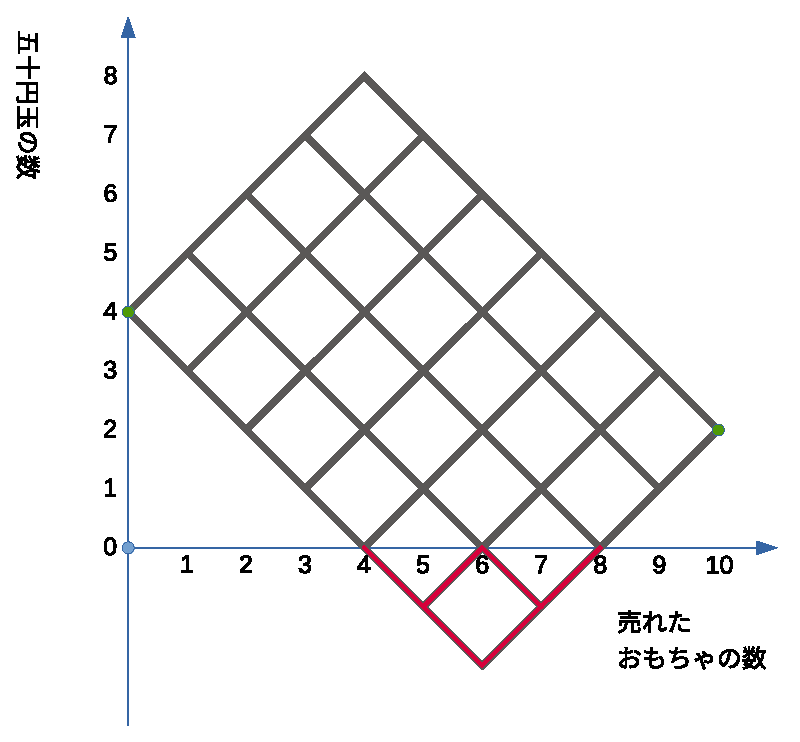
\includegraphics[width=5cm]{S030/Figs/Figure.change.p01.eps}
  \caption{お釣り玉の残数の変化経路図}
  \label{fig:S030/Figs/Figure.change.p01}
  \end{minipage}~
%\end{figure}
%%FFFFFFFFFFFFFFFFFFFFFFFFFFFFFFFFFFFFFFFFFFFFFFFFFFFFFFFFFFFFFFFFFFFFFF
%%FFFFFFFFFFFFFFFFFFFFFFFFFFFFFFFFFFFFFFFFFFFFFFFFFFFFFFFFFFFFFFFFFFFFFF
%\begin{figure}[b]
  \begin{minipage}[c]{.49\linewidth}  %{width}
  \centering
  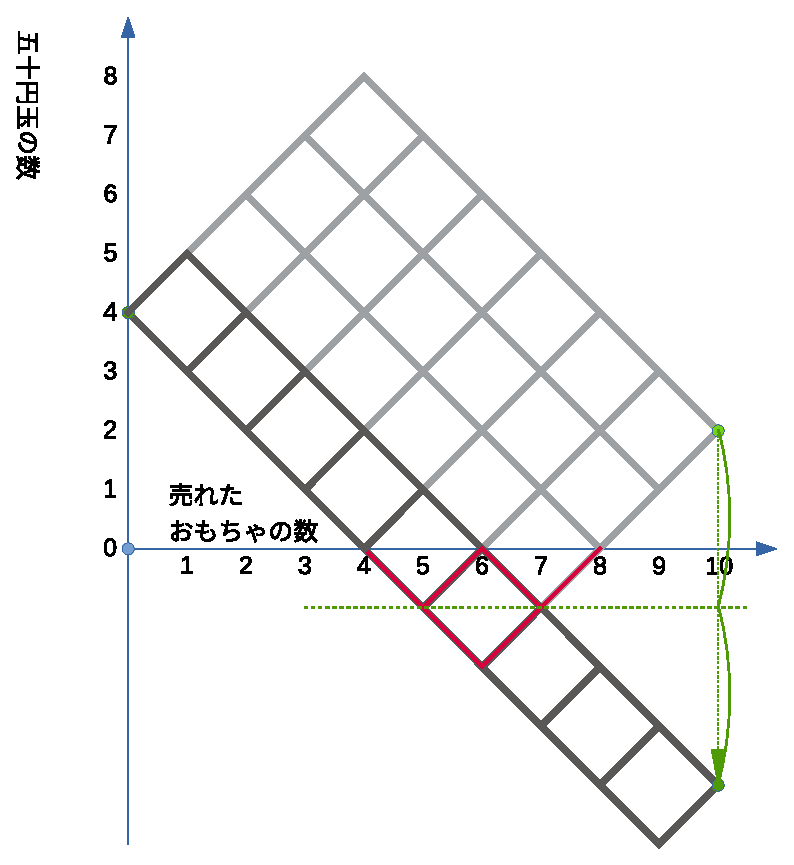
\includegraphics[width=5cm]{S030/Figs/Figure.change.p02.eps}
  \caption{お釣り玉が足らなくなる場合の残数の変化経路図}
  \label{fig:S030/Figs/Figure.change.p02}
  \end{minipage}
\end{figure}
%%FFFFFFFFFFFFFFFFFFFFFFFFFFFFFFFFFFFFFFFFFFFFFFFFFFFFFFFFFFFFFFFFFFFFFF


%%--------------------------------------------------
\subsubsection{一般化問題}
\label{sssec:お釣り:解答:一般化問題}
%% - - - - - - - - - - - - - - - - - - - - - - - - -

上記と同じ考え方をすると、
お釣りが足らなくなる場合の考えずに全ての経路を考えると、
$(0,m)$ から $(n,l)$ に至る斜めの碁盤目の経路となる。
この経路の数は
$n$ の候補の中から $\frac{n - (m-l)}{2}$ を順不同で選び出す場合の数であるので、
以下のように表せる。
  %%$$$$$$$$$$$$$$$$$$$$$$$$$$$$$$$$$$$$$$$$$$$$$$$$$$$$$$$$$$$$$$$$$$$$$$
  \begin{eqnarray}
    N_{\text{all}} & = & _{n}C_{\frac{n - (m-l)}{2}}
  \end{eqnarray}
  %%$$$$$$$$$$$$$$$$$$$$$$$$$$$$$$$$$$$$$$$$$$$$$$$$$$$$$$$$$$$$$$$$$$$$$$

一方、お釣りが足りなくなる経路の数は、
$(0,m)$ から $(n,-l-2)$ に至る斜めの碁盤目の経路となる。
この経路の数は
$n$ の候補の中から $\frac{n - (m+l+2)}{2}$ を順不同で選び出す場合の数であるので、
以下のように表せる。
  %%$$$$$$$$$$$$$$$$$$$$$$$$$$$$$$$$$$$$$$$$$$$$$$$$$$$$$$$$$$$$$$$$$$$$$$
  \begin{eqnarray}
    N_{\text{short}} & = & _{n}C_{\frac{n - (m+l+2)}{2}}
  \end{eqnarray}
  %%$$$$$$$$$$$$$$$$$$$$$$$$$$$$$$$$$$$$$$$$$$$$$$$$$$$$$$$$$$$$$$$$$$$$$$

よって、お釣りが足らなくならない経路の数は、
以下のように表すことができる。
  %%$$$$$$$$$$$$$$$$$$$$$$$$$$$$$$$$$$$$$$$$$$$$$$$$$$$$$$$$$$$$$$$$$$$$$$
  \begin{eqnarray}
    N_{\text{ans}} & = & N_{\text{all}} - N_{\text{short}}
  \\
      & = & _{n}C_{\frac{n - (m-l)}{2}} - _{n}C_{\frac{n - (m+l+2)}{2}}
  \end{eqnarray}
  %%$$$$$$$$$$$$$$$$$$$$$$$$$$$$$$$$$$$$$$$$$$$$$$$$$$$$$$$$$$$$$$$$$$$$$$
